\documentclass[10pt,twocolumn,a4paper]{article}
\usepackage[T1]{fontenc}
\usepackage{mathptmx}
\usepackage{amsmath,amssymb,amsthm}
\usepackage[a4paper,top=2.3cm,bottom=2.3cm,left=1.8cm,right=1.8cm,columnsep=0.7cm]{geometry}
\usepackage{graphicx,booktabs,xcolor}
\usepackage[font=small,labelfont=bf,labelsep=space,justification=justified,singlelinecheck=false]{caption}
\usepackage{titlesec}
\usepackage{fancyhdr}
\usepackage{microtype}
\usepackage[colorlinks=true,linkcolor=blue!55!black,citecolor=blue!55!black,urlcolor=blue!55!black]{hyperref}

% ---- Springer-like appearance -------------------------------------------------
\titleformat{\section}{\normalfont\bfseries\large}{\thesection}{0.6em}{}
\titleformat{\subsection}{\normalfont\bfseries}{\thesubsection}{0.6em}{}
\titlespacing*{\section}{0pt}{1.4ex plus .5ex}{0.9ex}
\titlespacing*{\subsection}{0pt}{1.1ex plus .4ex}{0.6ex}
\captionsetup[figure]{name=Fig.}
\setlength{\parindent}{1em}
\pagestyle{fancy}\fancyhf{}
\renewcommand{\headrulewidth}{0.4pt}
\fancyhead[L]{\small Preprint (2026)}
\fancyhead[R]{\small A. Suleman: Optimal lattices for a three-body power-law energy}
\fancyfoot[C]{\small\thepage}
\fancypagestyle{first}{\fancyhf{}\renewcommand{\headrulewidth}{0.4pt}\fancyhead[L]{\small Preprint\\ \small Mathematical Physics}\fancyfoot[C]{\small\thepage}}

\newtheorem{theorem}{Theorem}
\newtheorem{lemma}{Lemma}
\newtheorem{corollary}{Corollary}
\theoremstyle{definition}
\newtheorem{definition}{Definition}
\newtheorem{conjecture}{Conjecture}
\newtheorem{remark}{Remark}
\newcommand{\R}{\mathbb{R}}
\newcommand{\Z}{\mathbb{Z}}

\begin{document}
\twocolumn[{%
\thispagestyle{first}
\vspace*{0.4cm}
{\LARGE\bfseries Optimal lattices for a three-body power-law energy: steep-decay limits, computer-assisted proofs and the minima of the modular graph functions $\boldsymbol{C_{s,s,s}}$\par}
\vspace{0.5cm}
{\large\bfseries Ali Suleman$^{1,2}$\par}
\vspace{0.25cm}
{\footnotesize
$^1$ Fachrichtung Mathematik, Universit\"at des Saarlandes, 66123 Saarbr\"ucken, Germany\\
$^2$ Department of Mathematics, ETH Z\"urich, 8092 Z\"urich, Switzerland\par}
\vspace{0.35cm}
{\footnotesize Preprint, September 2026\par}
\vspace{0.6cm}
}]

\noindent\textbf{Abstract}\enspace
We study which Bravais lattice of fixed density minimises the three-body energy $T_\nu(\Lambda)=\sum'_{x,y\in\Lambda}(|x|\,|y|\,|x-y|)^{-\nu}$, the sum over all lattice triangles through the origin of the product of their side lengths to the power $-\nu$. In two dimensions $T_{2s}$ coincides, up to a factor, with the two-loop modular graph function $C_{s,s,s}(\tau)$. We prove that in the steep-decay limit $\nu\to\infty$ the minimisers converge to the rectangular lattice with aspect ratio $\sqrt{(\sqrt{17}-1)/2}$ in $d=2$, by solving exactly the associated max--min problem for the smallest triangle product, and to the body-centred cubic lattice in $d=3$, by a computer-assisted argument. For finite exponents we give computer-assisted proofs that $C_{2,2,2}$, $C_{3,3,3}$ and $C_{4,4,4}$ attain their minimum only at the square point $\tau=i$ (whereas $C_{1,1,1}$ is minimal at the hexagonal point), that the square lattice is the unique minimiser also for $\nu=5,7$, that the hexagonal lattice is the unique minimiser for $\nu=3.5$, and that the hexagonal and square energies cross in $(3.918364,3.918366)$. The proofs rest on a majorant series that bounds all Taylor coefficients of every summand uniformly in the lattice vectors. Numerically, the planar minimiser passes from hexagonal to square at $\nu^*\approx3.91836$ (first order) and from square to rectangular at $\nu_2=8.6063\pm0.0005$; in three dimensions BCC is optimal for all tested exponents, FCC loses local stability at $\nu_c=3.7521\pm0.0001$, and hcp is never optimal.

\medskip
\noindent\textbf{Keywords}\enspace Lattice energy minimisation $\cdot$ Three-body interactions $\cdot$ Modular graph functions $\cdot$ Computer-assisted proof $\cdot$ Max--min problems $\cdot$ Crystallisation

\section{Introduction}
Which periodic arrangement of points minimises a given interaction energy is one of the classical questions linking number theory, geometry and the physics of crystals. For \emph{pair} interactions a great deal is known: for completely monotone functions of the squared distance the hexagonal lattice is optimal in the plane among all lattices of fixed density \cite{Rankin,Cassels,Ennola,Diananda,Montgomery}, universal optimality has been established for $E_8$ and the Leech lattice \cite{CKMRV}, and phase transitions between optimal lattices have been classified for many two-term and ratio-type pair energies \cite{BST,Betermin2D,LuoWei}. In three dimensions the optimality of the face-centred cubic lattice for Epstein zeta functions (the Sarnak--Str\"ombergsson conjecture) has recently been claimed \cite{LuoWeiFCC}.

Much less is known for genuine \emph{many-body} energies. The simplest one is the product-form three-body power law
\begin{equation}\label{eq:T}
T_\nu(\Lambda)=\sum_{\substack{x,y\in\Lambda\setminus\{0\}\\ x\neq y}}\bigl(|x|\,|y|\,|x-y|\bigr)^{-\nu},
\end{equation}
which converges for $\nu>2d/3$. At $\nu=3$ it is the radial part of the Axilrod--Teller--Muto (ATM) triple-dipole energy; under the name \emph{three-body zeta function} it was introduced and evaluated for selected lattices and along the Bain path in \cite{RoblesNavarro}, and efficient algorithms for such many-body lattice sums were developed in \cite{BuchheitBusse,BuchheitRupp}. We stress that \eqref{eq:T} is a model energy: physical three-body dispersion carries an angular factor and always comes with pair terms. Our motivation is mathematical. In $d=2$, the energy $T_{2s}$ is (up to normalisation) the two-loop \emph{modular graph function} $C_{s,s,s}(\tau)$ from the low-energy expansion of genus-one string amplitudes \cite{DGV}; its minimum over the fundamental domain appears not to have been studied.

Two remarks delimit the content. First, $T_\nu$ is invariant under isometries, so the hexagonal and the square lattice (the elliptic fixed points $\rho=e^{i\pi/3}$ and $i$ of the modular group) are always critical points \cite{BetCrit}. The substance of the results below is \emph{global} minimality and the location of transitions. Second, the reduction of a steep-decay limit to a packing-type problem is standard for pair energies \cite{BST}; here it leads to a new max--min problem for triangles, related in spirit to three-point packing problems on the sphere \cite{Bilyk}.

\smallskip\noindent\textbf{Summary of results.} Fig.~\ref{fig:overview} summarises the planar picture.
\begin{itemize}\setlength\itemsep{1pt}
\item Theorem~\ref{thm:maxmin} solves exactly the planar max--min problem for the smallest triangle product; Theorem~\ref{thm:limit} deduces that minimisers of $T_\nu$ converge to a rectangular lattice with aspect ratio $y_\infty=\sqrt{(\sqrt{17}-1)/2}$.
\item Theorem~\ref{thm:3d} (computer-assisted) shows that in $d=3$ the body-centred cubic (BCC) lattice is the unique maximiser of the smallest triangle product; minimisers of $T_\nu$ converge to BCC.
\item Theorem~\ref{thm:finite} (computer-assisted) establishes the minimiser for the finite exponents $\nu\in\{3.5,4,5,6,7,8\}$; in particular $C_{2,2,2}$, $C_{3,3,3}$, $C_{4,4,4}$ are minimal only at $\tau=i$.
\item Sections~\ref{sec:numerics} and~\ref{sec:mixed} give the numerical phase diagrams with error bars, including hcp, unequal exponents and mixed pair plus three-body energies.
\end{itemize}

\begin{figure*}[t]
\centering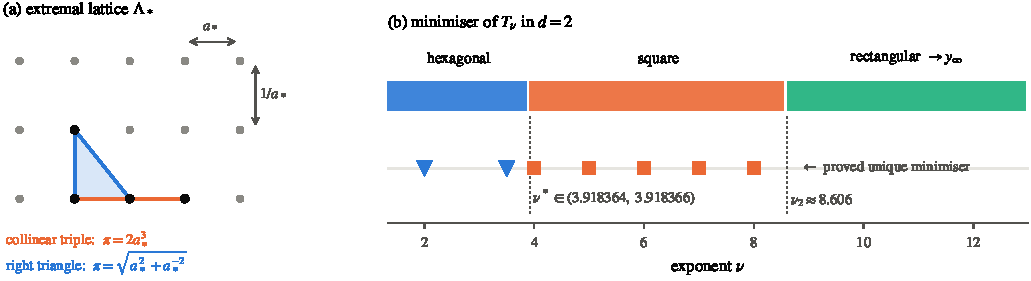
\includegraphics[width=0.92\textwidth]{figures/fig1_overview.pdf}
\caption{(a) The extremal lattice $\Lambda_*$ of Theorem~\ref{thm:maxmin}: the collinear triple (red) and the right triangle (blue) have the same side-length product $P_*$. (b) Minimiser of $T_\nu$ in $d=2$. Shaded regions: numerical phase diagram (Sect.~\ref{sec:numerics}); symbols: exponents at which the minimiser is established rigorously ($\nu=2$ classical, the others by Theorem~\ref{thm:finite}). For $\nu\to\infty$ the minimiser converges to $\Lambda_*$ (Theorem~\ref{thm:limit}).}
\label{fig:overview}
\end{figure*}

\section{Setting and the modular graph function}\label{sec:setting}
Throughout, lattices are Bravais lattices of unit covolume, considered up to isometry. For three pairwise distinct points $p,q,r$ put $\pi(p,q,r)=|p-q|\,|q-r|\,|r-p|$, and let
\[
P(\Lambda)=\min\{\pi(p,q,r):\ p,q,r\in\Lambda\ \text{pairwise distinct}\},
\]
the smallest triangle product; collinear triples are admitted. Every triple can be translated to contain the origin, hence
\begin{equation}\label{eq:lower}
T_\nu(\Lambda)\ \ge\ P(\Lambda)^{-\nu}.
\end{equation}
In $d=2$ we write $\Lambda_\tau=(\Z+\tau\Z)/\sqrt{\operatorname{Im}\tau}$ with $\tau=x+iy$ in the fundamental domain. The modular graph function of \cite{DGV} is
$C_{a,b,c}(\tau)=\sum_{p_1+p_2+p_3=0,\,p_i\neq0}\prod_i(\operatorname{Im}\tau/\pi|p_i|^2)^{a_i}$, $p_i\in\Z+\tau\Z$, and a direct comparison gives
\begin{equation}\label{eq:mgf}
C_{s,s,s}(\tau)=\pi^{-3s}\,T_{2s}(\Lambda_\tau).
\end{equation}
At $s=1$, Zagier's identity $C_{1,1,1}=E_3+\zeta(3)$ and the minimality of the Epstein zeta function at $\rho$ \cite{Rankin,Cassels,Ennola,Diananda} show that $C_{1,1,1}$ is minimal only at $\rho$. We verified \eqref{eq:mgf} numerically, and the identities $C_{1,1,1}=E_3+\zeta(3)$ and $C_{2,2,1}=\tfrac25E_5+\zeta(5)/30$ to relative accuracy $10^{-14}$ and $10^{-15}$ at five values of $\tau$ (Appendix~\ref{app:numerics}).

\section{The planar steep-decay limit}\label{sec:2d}
Let $a_*=((1+\sqrt{17})/8)^{1/4}\approx0.894563$, so that $4a_*^8=a_*^4+1$, and put
\[
P_*=2a_*^3=\sqrt{a_*^2+a_*^{-2}}\approx1.431734,\qquad \Lambda_*=a_*\Z\times a_*^{-1}\Z .
\]
The aspect ratio of $\Lambda_*$ is $y_\infty=a_*^{-2}=\sqrt{(\sqrt{17}-1)/2}\approx1.249621$.

\begin{theorem}\label{thm:maxmin}
For every lattice $\Lambda\subset\R^2$ of unit covolume, $P(\Lambda)\le P_*$, with equality if and only if $\Lambda$ is isometric to $\Lambda_*$.
\end{theorem}

\begin{lemma}\label{lem:red}
After a rotation and a reflection, $\Lambda$ has a basis $u=(a,0)$, $v=(p,a^{-1})$ with $a=\lambda_1(\Lambda)$, $0\le p\le a/2$ and $|v|\ge a$; moreover $a^4\le4/3$.
\end{lemma}
\begin{proof}
Lagrange--Gauss reduction; the bound is Hermite's constant $\gamma_2=2/\sqrt3$.
\end{proof}

\begin{lemma}\label{lem:upper}
In the notation of Lemma~\ref{lem:red}, $P(\Lambda)\le G(a):=\min\{2a^3,\sqrt{a^2+a^{-2}}\}$, and $\pi(0,u,v)\le\sqrt{a^2+a^{-2}}$ with equality if and only if $p=0$.
\end{lemma}
\begin{proof}
The collinear triple $(0,u,2u)$ gives $2a^3$. For $(0,u,v)$ we have $\pi^2=a^2(p^2+k)((a-p)^2+k)$ with $k=a^{-2}$. With $m=p(a-p)\in[0,a^2/4]$ and $p^2+(a-p)^2=a^2-2m$,
\[
(p^2+k)((a-p)^2+k)=(ka^2+k^2)+m(m-2k).
\]
Since $a^4<8$, $m\le a^2/4<2k$, so the last term is $\le0$, with equality iff $m=0$, i.e.\ $p=0$. Hence $\pi^2\le a^2(ka^2+k^2)=a^2+a^{-2}$.
\end{proof}

\begin{lemma}\label{lem:G}
For $0<a\le(4/3)^{1/4}$, $G(a)\le P_*$ with equality iff $a=a_*$.
\end{lemma}
\begin{proof}
For $a\le a_*$, $G(a)\le2a^3\le2a_*^3$. The function $g(a)=a^2+a^{-2}$ decreases on $(0,1]$ and increases on $[1,\infty)$. For $a_*<a\le1$, $G(a)\le\sqrt{g(a)}<\sqrt{g(a_*)}=P_*$. For $1\le a\le(4/3)^{1/4}$, $g(a)\le\frac{2}{\sqrt3}+\frac{\sqrt3}{2}=\frac{7}{2\sqrt3}$ and $(\frac{7}{2\sqrt3})^2=\frac{49}{12}<16(\frac{1+\sqrt{17}}{8})^3=P_*^4$.
\end{proof}

\begin{lemma}\label{lem:star}
$P(\Lambda_*)=P_*$.
\end{lemma}
\begin{proof}
The triples in Fig.~\ref{fig:overview}(a) give $P(\Lambda_*)\le P_*$. Collinear triples lie on a lattice line with spacing $s\ge a_*$ and have $\pi=s^3(k-j)(l-k)(l-j)\ge2s^3\ge P_*$. A non-collinear lattice triangle has area $\ge\frac12$; with side lengths $d_1\le d_2\le d_3$ and $\gamma$ the angle between the two shorter sides, $d_1d_2\ge d_1d_2\sin\gamma\ge1$, hence $\pi\ge d_3$. The only vectors of $\Lambda_*$ shorter than $D=\sqrt{a_*^2+a_*^{-2}}$ are $\pm u,\pm v$ with $u=(a_*,0)$, $v=(0,a_*^{-1})$: for $(ma_*,na_*^{-1})$ with $n\neq0$ one gets $m=0$ and $n^2<1+a_*^4<2$, and for $n=0$, $m^2<1+y_\infty^2<4$. They span two directions, whereas the three sides of a triangle are pairwise linearly independent. Thus $d_3\ge D=P_*$.
\end{proof}

\begin{proof}[Proof of Theorem~\ref{thm:maxmin}]
Lemmas~\ref{lem:red}--\ref{lem:G} give $P(\Lambda)\le G(a)\le P_*$. Equality forces $a=a_*$ and $\pi(0,u,v)\ge P_*=\sqrt{a_*^2+a_*^{-2}}$, hence $p=0$ by Lemma~\ref{lem:upper}, i.e.\ $\Lambda=\Lambda_*$. The converse is Lemma~\ref{lem:star}.
\end{proof}

\begin{theorem}\label{thm:limit}
For every $\nu>4/3$, $T_\nu$ attains its minimum among planar lattices of unit covolume. If $\Lambda_\nu$ is any minimiser, then $\Lambda_\nu\to\Lambda_*$ up to isometries as $\nu\to\infty$, and $(\min T_\nu)^{1/\nu}\to1/P_*$. Equivalently, minimisers $\tau_s$ of $C_{s,s,s}$ on the fundamental domain satisfy $\tau_s\to i\,y_\infty$ as $s\to\infty$.
\end{theorem}
\begin{proof}
$P$ is continuous and $P(\Lambda)\le2\lambda_1(\Lambda)^3$; $T_\nu$ is lower semicontinuous as a sum of non-negative continuous functions. By \eqref{eq:lower}, sublevel sets of $T_\nu$ lie in $\{\lambda_1\ge\varepsilon\}$, compact by Mahler's criterion, so minimisers exist. Every term of $T_\nu(\Lambda_*)$ has $\pi\ge P_*$, whence $T_\nu(\Lambda_*)\le C\,P_*^{-\nu}$ for $\nu\ge\nu_0$ with $C=T_{\nu_0}(\Lambda_*)P_*^{\nu_0}$. With \eqref{eq:lower},
$P(\Lambda_\nu)^{-\nu}\le T_\nu(\Lambda_\nu)\le T_\nu(\Lambda_*)\le CP_*^{-\nu}$, so $P_*\ge P(\Lambda_\nu)\ge C^{-1/\nu}P_*\to P_*$. The $\Lambda_\nu$ lie in a compact set; every limit point has $P=P_*$ and is $\Lambda_*$ by Theorem~\ref{thm:maxmin}. The statement for $C_{s,s,s}$ follows from \eqref{eq:mgf}.
\end{proof}
The numerical minimisers for finite $\nu$ (Sect.~\ref{sec:numerics}) approach $\Lambda_*$ monotonically: the optimal aspect ratio is $1.056$, $1.100$, $1.141$, $1.170$, $1.194$ and $1.215$ at $\nu=9,10,12,15,20,30$. A random test on $2\cdot10^4$ lattices confirmed the bound of Lemma~\ref{lem:upper}, and a grid maximisation of $P$ located the maximum at $\tau\approx1.2475\,i$.

\section{Three dimensions}\label{sec:3d}
In $d=3$ the energy converges for $\nu>2$. For BCC of unit covolume $P(\mathrm{BCC})=3/2$, attained by isosceles triangles with two nearest-neighbour sides and one second-neighbour side; in contrast $P(\mathrm{FCC})=P(\mathrm{SC})=P(\mathrm{hcp})=\sqrt2$.

\begin{theorem}[computer-assisted]\label{thm:3d}
For every lattice $\Lambda\subset\R^3$ of unit covolume, $P(\Lambda)\le3/2$, with equality iff $\Lambda$ is isometric to BCC. Consequently, for $\nu>2$ minimisers of $T_\nu$ exist and converge to BCC as $\nu\to\infty$, with $(\min T_\nu)^{1/\nu}\to2/3$.
\end{theorem}
Let $G=B^{\mathsf T}B$ be the Gram matrix of a basis, normalised by $G_{11}=\lambda_1^2=1$, and $Q(G)=P(\Lambda)/\sqrt{\det G}$ (scale invariant). The remaining entries $q=(g_{22},g_{33},g_{12},g_{13},g_{23})$ are the parameters.

\begin{lemma}\label{lem:region}
Every lattice has, up to isometry and scaling, a Gram matrix in the region $\mathcal R$ given by $1\le g_{22}\le g_{33}$, $0\le g_{12},g_{13}\le\frac12$, $|g_{23}|\le g_{22}/2$ and $1+g_{22}+2(\varepsilon_1\varepsilon_2g_{12}+\varepsilon_1g_{13}+\varepsilon_2g_{23})\ge0$ for $\varepsilon_i=\pm1$. On $\mathcal R$, $\det G\ge g_{22}g_{33}/4$; hence $Q<3/2$ whenever $g_{22}g_{33}>64/9$.
\end{lemma}
\begin{proof}
Take a Minkowski-reduced basis and flip the signs of $b_2,b_3$. The triangle $(0,b_1,b_2)$ is acute, so the covering radius of $L_2=\Z b_1+\Z b_2$ is its circumradius $\rho$, with $\rho^2=g_{22}|b_2-b_1|^2/(4(g_{22}-g_{12}^2))\le(1+g_{22})/3$. Minkowski reduction places the projection of $b_3$ onto the plane of $L_2$ in its Voronoi cell, so the height $h$ of $b_3$ satisfies $h^2\ge g_{33}-\rho^2\ge g_{33}/3$, and $\det G=(g_{22}-g_{12}^2)h^2\ge g_{22}g_{33}/4$. The collinear triple $(0,b_1,2b_1)$ gives $Q\le2/\sqrt{\det G}$.
\end{proof}
Within $\mathcal R$, BCC has the single representative $q_0=(1,1,\frac13,\frac13,-\frac13)$, found by enumerating unimodular changes of basis.

\begin{lemma}[local lemma]\label{lem:local3}
For a triangle $t=(0,m,n)$ put $f_t(q)=\sqrt{\ell_m\ell_n\ell_{m-n}/\det G}$ with $\ell_v=v^{\mathsf T}Gv$. At $q_0$ exactly 36 triangles are active, $f_t(q_0)=3/2$, and their gradients take 6 distinct values whose convex hull contains the origin at distance $c=0.13887$ from its boundary. On $q_0+[-r,r]^5$ with $r=0.007$, interval arithmetic gives $\|\nabla^2f_t\|_F\le M=14.92$ for all active $t$. Hence $\min_tf_t(q_0+\delta)\le\frac32-c|\delta|+\frac M2|\delta|^2<\frac32$ for $0<|\delta|\le\sqrt5\,r=0.0157<2c/M=0.0186$.
\end{lemma}

\noindent\emph{Branch and bound.} On a box $B$ of parameters each $\ell_v$ is linear in $q$ and $\det G$ is a cubic polynomial, so
$Q\le\min_{t\in S}(\prod\max_B\ell)^{1/2}(\min_B\det G)^{-1/2}$ for any set $S$ of candidate triangles; we use all $(0,m,n)$ with $m,n\in\{-1,0,1\}^3$ and the collinear $(0,m,2m)$. Starting from the compact box $[1,\frac83]\times[1,\frac{64}{9}]\times[0,\frac12]^2\times[-\frac43,\frac43]$, boxes are discarded when they violate a constraint of $\mathcal R$, lie in $q_0+[-r,r]^5$, or have upper bound $<3/2$, and bisected otherwise. The run terminates after $9.93\cdot10^6$ boxes with every box certified. With Lemmas~\ref{lem:region} and~\ref{lem:local3} this proves $Q\le3/2$ on $\mathcal R$ with equality only at $q_0$. The convergence statement follows as in Theorem~\ref{thm:limit}.

\section{Finite exponents: computer-assisted proofs}\label{sec:finite}
\begin{theorem}[computer-assisted]\label{thm:finite}
Among planar lattices of unit covolume, the square lattice is the unique minimiser of $T_\nu$ for $\nu\in\{4,5,6,7,8\}$, and the hexagonal lattice is the unique minimiser for $\nu=3.5$. In particular $C_{2,2,2}$, $C_{3,3,3}$ and $C_{4,4,4}$ attain their minimum on the fundamental domain only at $\tau=i$. Moreover $T_\nu(\Z^2)-T_\nu(\Lambda_\rho)$ changes sign in $(3.918364,3.918366)$.
\end{theorem}
Together with the case $s=1$ and Theorem~\ref{thm:limit}, the minimiser of $C_{s,s,s}$ is thus $\rho$ for $s=1$, $i$ for $s=2,3,4$, and tends to $i\,y_\infty$ as $s\to\infty$.

\smallskip\noindent\emph{A universal majorant.} For $v=(m,n)$ and $\tau=x+iy$ let $\ell_v=|m+n\tau|^2/y$, so that $T_\nu=\sum\prod_{\rm sides}\ell^{-s}$ with $s=\nu/2$. Around $(x_0,y_0)$ put $A=a/y_0$, $B=b/y_0$. A short computation gives
\[
\frac{\ell_v(x_0+a,y_0+b)}{\ell_v(x_0,y_0)}=1+\frac{(2\alpha^2-1)B+2\alpha\beta A+\alpha^2(A^2+B^2)}{1+B},
\]
where $\alpha^2+\beta^2=1$ depend on $v$. Coefficientwise, therefore,
$\ell/\ell_0-1\ll\hat\varepsilon:=(A+B+A^2+B^2)/(1-B)$, and every triangle term $t$ satisfies $t/t_0\ll(1-\hat\varepsilon)^{-3s}$, \emph{uniformly in the lattice vectors}. Consequently all Taylor coefficients of $T_\nu$ at $\tau_0$ are bounded by $T_\nu(\tau_0)$ times the coefficients $\hat G_{ij}$ of $(1-\hat\varepsilon)^{-3s}$. This yields explicit Taylor remainders and explicit bounds for the terms omitted by a finite truncation.

\smallskip\noindent\emph{Proof structure.} Let $\tau_0\in\{i,\rho\}$ be the candidate.
(i) For $y>Y_0$ the collinear triples along the vector $1$ give $T_\nu(\tau)\ge y^{3s}\sum_{j\neq k}(|j||k||j-k|)^{-2s}>T_\nu(\tau_0)$.
(ii) Local lemma: the reflections fixing $\tau_0$ ($x\mapsto-x$ and $\tau\mapsto1/\bar\tau$ at $i$; $x\mapsto1-x$ and the order-three rotation at $\rho$) force $c_{10}=c_{01}=c_{11}=c_{30}=c_{12}=0$ in the Taylor expansion. With rigorous enclosures of $c_{20},c_{02},c_{21},c_{03}$ and the majorant remainder, $T(\tau_0+\delta)-T(\tau_0)\ge A^2(c_{20}-|c_{21}|r-\varrho)+B^2(c_{02}-|c_{03}|r-\varrho)>0$ for $0<\max(|A|,|B|)\le r_{\rm loc}$, where $\varrho=T\sum_{i+j\ge4}\hat G_{ij}r^{i+j-2}$.
(iii) The rest of $[0,\frac12]\times[0.8,Y_0]$ is covered by boxes on which the second-order Taylor polynomial at the centre, with rigorous coefficient enclosures, minus the majorant remainder exceeds an upper bound for $T(\tau_0)$.
All coefficients are computed from cube-truncated sums ($R=40$) by direct, non-FFT convolution, with an explicit tail bound and a rounding margin. Table~\ref{tab:finite} lists the data.

\begin{table}[t]
\caption{Data of the computer-assisted proofs of Theorem~\ref{thm:finite}.}
\label{tab:finite}\centering\footnotesize
\setlength{\tabcolsep}{3.2pt}
\begin{tabular}{@{}cccccc@{}}\toprule
$\nu$ & point & $T_\nu(\tau_0)$ (enclosure) & $c_{20}\ge$ & $r_{\rm loc}$ & boxes\\\midrule
3.5 & $\rho$ & $[9.77234289489,\,9.77240888476]$ & 2.1286 & 0.0072 & 363\\
4 & $i$ & $[7.58266977207,\,7.58267002471]$ & 0.4369 & 0.0031 & 531\\
5 & $i$ & $[4.83802684613,\,4.83802684730]$ & 2.5822 & 0.0070 & 303\\
6 & $i$ & $[3.24997431212,\,3.24997431277]$ & 4.2719 & 0.0076 & 307\\
7 & $i$ & $[2.23344617456,\,2.23344617501]$ & 5.3445 & 0.0050 & 323\\
8 & $i$ & $[1.55240121242,\,1.55240121273]$ & 5.8308 & 0.0026 & 385\\\bottomrule
\end{tabular}
\end{table}

The crossing statement uses the same tail bound. The cube sums at $R=100$ are evaluated by direct convolution and give $T_\nu(\Z^2)-T_\nu(\Lambda_\rho)\in[2.36,2.77]\cdot10^{-7}$ at $\nu=3.918364$ and $\in[-3.41,-3.00]\cdot10^{-7}$ at $\nu=3.918366$.

\begin{remark}[status of the computer-assisted parts]
The local lemma of Sect.~\ref{sec:3d} uses rigorous interval arithmetic. The branch-and-bound parts use IEEE double precision with explicit safety margins: $10^{-9}$ relative on bounds, $10^{-12}$ absolute on determinants, and $10^{-10}$ relative on sums. These exceed the rounding errors of the few operations per bound, and of sequential sums of at most $2\cdot10^4$ positive terms, by several orders of magnitude. As sanity checks, the three-dimensional box bounds were compared with brute-force values at 1200 random points without a single violation, and the prover fails, as it must, when asked to certify $Q<1.49$. A re-run in full interval arithmetic is straightforward.
\end{remark}

The same method did not succeed for the hexagonal lattice at $\nu=3$. Close to $\nu=d$ the truncation tail decays only like $R^{-4}$, and at $R=40$ the error exceeds the energy gap next to $\rho$.

\section{Numerical phase diagram}\label{sec:numerics}
The numerical results use an independent reference summation, described in Appendix~\ref{app:numerics}. It agrees with the library of \cite{BuchheitRupp} to better than $2\cdot10^{-10}$ relative in 55 test cases and reproduces the published values of \cite{RoblesNavarro} at $\nu=3$.

\smallskip\noindent\textbf{Two dimensions.} A global search over the fundamental domain gives the following picture (Figs.~\ref{fig:energy}--\ref{fig:landscape}).
\begin{itemize}\setlength\itemsep{1pt}
\item For $4/3<\nu<\nu^*$ the minimiser is hexagonal. For $1.4\le\nu\le1.9$ the hexagonal lattice is the best candidate with a stability of $10^{-8}$ across cut-off sets, using an extrapolation ansatz with the two exponent families $R^{d-2\nu}$ and $R^{2d-3\nu}$.
\item At $\nu^*=3.9183649026$ there is a first-order transition to the square lattice. Both lattices are local minima for $3.80632<\nu<4.27848$ (errors below $6\cdot10^{-5}$), and along the arc $|\tau|=1$ the barrier is $0.14\%$.
\item At $\nu_2=8.6063\pm0.0005$ the square lattice becomes unstable towards rectangular deformations, and the optimal aspect ratio then grows continuously towards $y_\infty$.
\end{itemize}
Error bars are the spread over three finite-difference steps and two cut-off sets.
\begin{conjecture}
In $d=2$ the minimiser of $T_\nu$ is hexagonal for $4/3<\nu<\nu^*$, square for $\nu^*<\nu\le\nu_2$, and rectangular with aspect ratio increasing from $1$ to $y_\infty$ for $\nu>\nu_2$.
\end{conjecture}

\begin{figure}[t]
\centering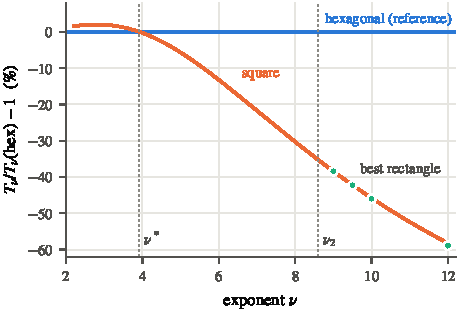
\includegraphics[width=\columnwidth]{figures/fig_2d_energy_difference.pdf}
\caption{Relative energy of the square lattice (line) and of the best rectangular lattice (dots) with respect to the hexagonal lattice. The zeros mark the two transitions.}
\label{fig:energy}
\end{figure}

\begin{figure}[t]
\centering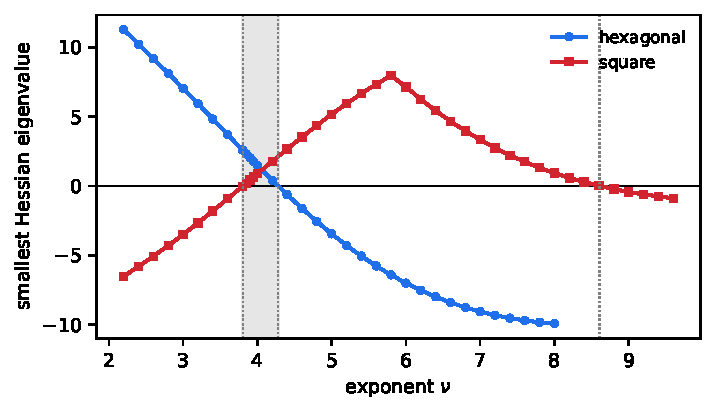
\includegraphics[width=\columnwidth]{figures/fig_2d_stability.pdf}
\caption{Smallest Hessian eigenvalue of $T_\nu$ at the hexagonal and at the square point. Grey: both are local minima (first-order transition). Right: loss of stability of the square lattice at $\nu_2$.}
\label{fig:stability}
\end{figure}

\begin{figure*}[t]
\centering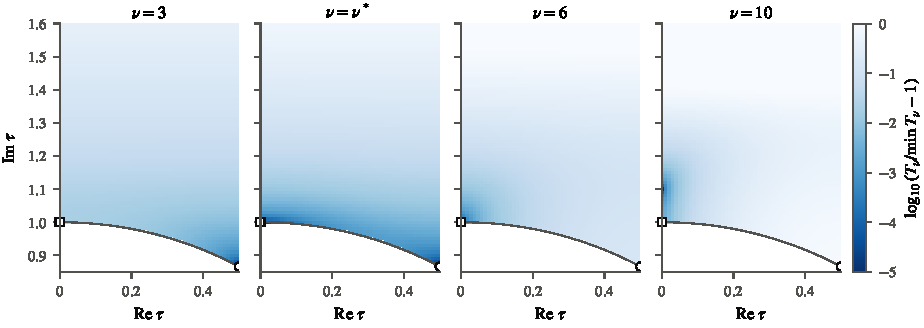
\includegraphics[width=0.85\textwidth]{figures/fig_2d_landscape.pdf}
\caption{Energy landscape $\log_{10}(T_\nu/\min T_\nu-1)$ on the fundamental domain for four exponents. Circle: hexagonal point; square: square point. At $\nu=10$ the minimum lies on the imaginary axis above $\tau=i$.}
\label{fig:landscape}
\end{figure*}

\smallskip\noindent\textbf{Unequal exponents.} Replacing the exponent of the side $|x-y|$ by $\mu$ gives, up to normalisation, $C_{\nu/2,\nu/2,\mu/2}$. The curve of Fig.~\ref{fig:overview}(b) then becomes a phase map (Fig.~\ref{fig:unequal}). The square phase occupies a broad band around the diagonal; for $4\le\nu\le5.5$ the hexagonal lattice returns at large $\mu$; the rectangular phase appears only for $\nu\gtrsim9$ in a window $8.5\lesssim\mu\lesssim11$. No rhombic or oblique minimiser was found.

\begin{figure}[t]
\centering
\includegraphics[width=0.92\columnwidth]{figures/fig_e3_phase_map.pdf}
\caption{Minimiser for the exponents $(\nu,\nu,\mu)$ on a grid of spacing $0.5$. Dashed: equal exponents.}
\label{fig:unequal}
\end{figure}

\smallskip\noindent\textbf{Three dimensions.} A global search over all Bravais lattices used 67 starts per exponent (FCC, BCC, SC and 64 random), Nelder--Mead and accurate re-evaluation. It returned BCC as the best lattice, to $10^{-9}$ relative, for every tested $\nu\in\{3.2,3.5,4,4.5,5,6,8,12\}$; between 87\% and 100\% of the starts converged to BCC. For $2.2\le\nu\le2.8$ the ordering BCC $<$ FCC $<$ SC persists. The curvature of $T_\nu$ at FCC along the Bain path changes sign at $\nu_c=3.7521\pm0.0001$, so FCC is a saddle point for larger $\nu$. Optimised over $c/a\in[1.45,1.85]$, hcp lies slightly above FCC for all tested $\nu$; at $\nu=4.5$, for example, the values are $17.9724$ against $17.9624$, while BCC gives $17.7406$. BCC is stationary along the Bain path for every exponent \cite{RoblesNavarro}.

\section{Mixed pair and three-body energies}\label{sec:mixed}
To connect with physically motivated energies we consider
$E_\lambda=Z_\nu+\lambda T_\nu$ at unit density. Here $Z_\nu=\sum'|x|^{-\nu}$ is the Epstein (Riesz) pair energy, evaluated exactly with \cite{EpsteinLib}, and $\lambda=c_3/c_2$. In $d=3$, among FCC, BCC, hcp$(c/a)$ and the Bain family, the minimiser jumps directly from FCC to BCC at $\lambda_c(\nu)\approx0.049$, $0.065$, $0.103$, $0.289$ for $\nu=3.5$, $4.5$, $6$, $9$; hcp is never optimal. In $d=2$ the minimiser jumps from hexagonal to square at $\lambda_c\approx1.86$, $1.04$, $1.51$ for $\nu=4.5$, $6$, $9$, with a further transition to a rectangular lattice at very large $\lambda$ for $\nu=9$. For $\nu<\nu^*$ both terms favour the hexagonal lattice (Fig.~\ref{fig:mixed}).

\begin{figure}[t]
\centering
\includegraphics[width=0.95\columnwidth]{figures/fig_e4_lambda_c.pdf}
\caption{Critical ratio $\lambda_c=c_3/c_2$ of the mixed energy $Z_\nu+\lambda T_\nu$.}
\label{fig:mixed}
\end{figure}

\section{Discussion}\label{sec:discussion}
A purely three-body repulsion of product type selects different lattices than pair repulsion does. In the plane it penalises the equilateral triangles of the hexagonal lattice once the decay is steep enough. In space it favours BCC, whose smallest triangles are isosceles with one second-neighbour side, over the close-packed FCC and hcp. The steep-decay limits reduce to max--min problems for triangles. The planar one has the closed-form answer of Theorem~\ref{thm:maxmin}; the spatial one we solved by a computer-assisted argument. Through \eqref{eq:mgf} the planar results translate into statements on the minima of the modular graph functions $C_{s,s,s}$.

Several questions remain open. (i) A proof of the full planar phase diagram, in particular hexagonal optimality for all $\nu<\nu^*$, would require the finite-$\nu$ method on continua of exponents and sharper tail bounds near $\nu=d$. (ii) An analytic proof of Theorem~\ref{thm:3d} is missing. (iii) Physically relevant three-body energies include the angular ATM factor; the mixed energies of Sect.~\ref{sec:mixed} are only a first step. (iv) The rectangular phase suggests that, for $\nu>\nu_2$, the minimiser lies on the imaginary axis for all larger $\nu$; this is supported numerically but unproven.

\section*{Declarations}
\noindent\textbf{Acknowledgements}\enspace Computations, literature searches and parts of the manuscript were prepared with the assistance of the AI system Claude (Anthropic). The author checked the mathematical arguments and is responsible for the content. Lattice sums were cross-checked against the Graph Zeta Library \cite{BuchheitRupp} and EpsteinLib \cite{EpsteinLib}.

\smallskip\noindent\textbf{Data availability}\enspace All scripts, raw data and logs, including the branch-and-bound provers and their test suites, are available from the author on request.

\smallskip\noindent\textbf{Competing interests}\enspace The author declares no competing interests.

\appendix
\section{Numerical methods and error control}\label{app:numerics}
\noindent\emph{Reference summation.} $T_\nu$ is summed over all integer labels in the cube $[-R,R]^d$ for the two free vertices, with the kernel of the third side on $[-2R,2R]^d$. The inner convolution is evaluated by FFT for exploratory computations and by direct convolution in the rigorous parts. The truncation error is dominated by configurations with one distant vertex and decays like $R^{d-2\nu}$ for $\nu>d$. For $2d/3<\nu\le d$ it decays like $R^{2d-3\nu}$ (with logarithms at $\nu=d$); Richardson extrapolation uses the corresponding exponents.

\smallskip\noindent\emph{Tail bound.} A term is missing only if a free vertex $x$ lies outside the cube. For fixed $x$, $\sum_y|y|^{-\nu}|x-y|^{-\nu}\le2(|x|/2)^{-\nu}Z_\nu$, and $|Am|\ge\sigma_{\min}(A)|m|_\infty$, whence
$0\le T-T_R\le2^{\nu+2}Z_\nu\,8\sigma_{\min}^{-2\nu}R^{2-2\nu}/(2\nu-2)$ in $d=2$.

\smallskip\noindent\emph{Non-Bravais structures.} For a crystal $\bigcup_j(L+s_j)$ the per-atom energy decomposes into sums $\sum_mF_{ij}(m)(F_{ik}*G_{jk})(m)$ over the Bravais lattice $L$. The implementation reproduces the FCC value with a four-atom cubic basis to $10^{-10}$.

\smallskip\noindent\emph{Validation.} Besides the agreement with \cite{BuchheitRupp,RoblesNavarro} mentioned above, the reference summation reproduces the identities $C_{1,1,1}=E_3+\zeta(3)$ (with logarithmic extrapolation, since all exponents equal $d$) and $C_{2,2,1}=\frac25E_5+\frac{\zeta(5)}{30}$ \cite{DGV} to $10^{-14}$ and $10^{-15}$.

\begin{thebibliography}{99}\footnotesize
\bibitem{Rankin} R.A. Rankin, A minimum problem for the Epstein zeta-function. Proc. Glasgow Math. Assoc. \textbf{1}, 149--158 (1953)
\bibitem{Cassels} J.W.S. Cassels, On a problem of Rankin about the Epstein zeta-function. Proc. Glasgow Math. Assoc. \textbf{4}, 73--80 (1959)
\bibitem{Ennola} V. Ennola, A lemma about the Epstein zeta-function. Proc. Glasgow Math. Assoc. \textbf{6}, 198--201 (1964)
\bibitem{Diananda} P.H. Diananda, Notes on two lemmas concerning the Epstein zeta-function. Proc. Glasgow Math. Assoc. \textbf{6}, 202--204 (1964)
\bibitem{Montgomery} H.L. Montgomery, Minimal theta functions. Glasgow Math. J. \textbf{30}, 75--85 (1988)
\bibitem{CKMRV} H. Cohn, A. Kumar, S.D. Miller, D. Radchenko, M. Viazovska, Universal optimality of the $E_8$ and Leech lattices and interpolation formulas. Ann. Math. \textbf{196}, 983--1082 (2022)
\bibitem{BST} L. B\'etermin, L. \v{S}amaj, I. Trav\v{e}nec, arXiv:2107.14020
\bibitem{Betermin2D} L. B\'etermin, L. \v{S}amaj, I. Trav\v{e}nec, arXiv:2312.01395
\bibitem{LuoWei} S. Luo, J. Wei, arXiv:2004.13882
\bibitem{LuoWeiFCC} S. Luo, J. Wei, arXiv:2609.17356 (2026)
\bibitem{RoblesNavarro} A. Robles-Navarro, S. Cooper, A.A. Buchheit, J.T. Busse, A. Burrows, O.R. Smits, P. Schwerdtfeger, J. Chem. Phys. \textbf{163}, 094104 (2025). arXiv:2504.07338
\bibitem{BuchheitBusse} A.A. Buchheit, J.T. Busse, An Epstein zeta method for many-body lattice sums. arXiv:2504.11989
\bibitem{BuchheitRupp} A.A. Buchheit, A. Rupp, arXiv:2609.18918 (2026); Graph Zeta Library, \url{https://github.com/graph-zeta/gzl}
\bibitem{EpsteinLib} A.A. Buchheit et al., EpsteinLib. arXiv:2412.16317
\bibitem{DGV} E. D'Hoker, M.B. Green, P. Vanhove, On the modular structure of the genus-one type II superstring low energy expansion. JHEP \textbf{08}, 041 (2015). arXiv:1502.06698
\bibitem{BetCrit} L. B\'etermin, arXiv:1611.07798
\bibitem{Bilyk} D. Bilyk et al., arXiv:2303.12283
\end{thebibliography}
\end{document}
